% !TeX root = 0_TCC.tex
% Resultados do teste original das categorias gerais. Não inclui reavaliação corrigida.
\begingroup
\justifying
\setlength{\parindent}{1.25cm}
\setlength{\parskip}{0pt}
\setlength{\emergencystretch}{2em}
\onehalfspacing
\renewcommand{\tablename}{Tabela}
\phantomsection
\addcontentsline{toc}{section}{4 RESULTADOS E DISCUSSÃO}
\noindent\textbf{4 RESULTADOS E DISCUSSÃO}\par
\nobreak\vspace{\baselineskip}\nobreak

Este capítulo apresenta os resultados do modelo YOLO26n treinado para detectar instrumentos e contar os objetos de sete categorias gerais. A análise procura responder em quais condições essa abordagem apresentou resultados favoráveis e quais dificuldades ainda limitam sua aplicação. Para isso, são examinados o aprendizado durante o treinamento, a localização dos objetos, a contagem por imagem e os exemplos de acertos e falhas observados no teste.

A avaliação utilizou 1.008 imagens reservadas para teste, com 1.377 objetos anotados: 559 fotografias do HU-UEL e 449 imagens de fontes da internet. Esses dados foram mantidos separados das 8.304 imagens de treinamento e das 1.015 imagens de validação. Os resultados a seguir se referem às categorias gerais, como pinças e tesouras, e não à distinção entre todos os instrumentos específicos que compõem cada categoria. Assim, identificar uma pinça como pertencente à categoria correta não significa, por si só, reconhecer se ela é uma Kelly, uma Kocher ou outro instrumento desse grupo.

\vspace{\baselineskip}
\phantomsection
\addcontentsline{toc}{subsection}{4.1 Evolução do treinamento}
\noindent\textbf{4.1 Evolução do treinamento}\par
\nobreak\vspace{\baselineskip}\nobreak

O treinamento foi concluído em 50 épocas, com duração aproximada de 8 horas e 43 minutos no Mac mini M4 com 16 GB de memória. Em cada época, o modelo percorreu o conjunto de treinamento e, em seguida, foi avaliado no conjunto de validação. Essa avaliação intermediária permitiu acompanhar o aprendizado sem utilizar o conjunto de teste para escolher os pesos do modelo.

A Figura~\ref{fig:res-treinamento} apresenta dois aspectos dessa evolução. À esquerda, as medidas de precisão média das detecções aumentam ao longo das épocas. À direita, diminui a perda de localização, que expressa o desajuste entre as caixas previstas e as caixas de referência utilizadas pelo algoritmo. A redução dessa perda indica que o treinamento passou a produzir delimitações mais próximas das anotações, embora ela não deva ser interpretada como uma porcentagem de acertos.

\begin{figure}[htbp]
\centering
\caption{Evolução das métricas de validação e da perda de localização durante o treinamento}
\label{fig:res-treinamento}
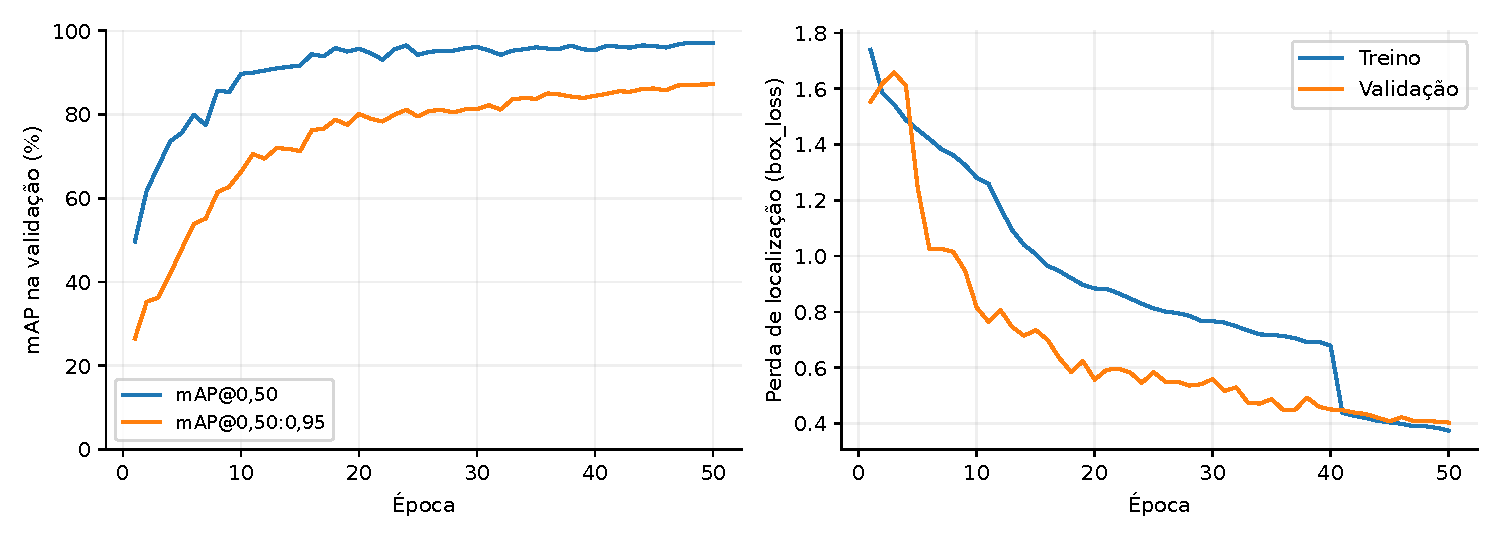
\includegraphics[width=\linewidth]{figuras/resultados_evolucao_treinamento.pdf}
\par\smallskip{\footnotesize Fonte: elaboração própria, com base nos registros do treinamento.\par}
\end{figure}



Na última época, a validação alcançou mAP@0,50 de 97,02\% e mAP@0,50:\allowbreak{}0,95 de 87,20\%. Este último foi o maior valor registrado nas 50 épocas. O checkpoint \texttt{best.pt}, selecionado com base nos resultados de validação, foi utilizado na avaliação do conjunto de teste. A diferença entre as duas medidas é esperada: a primeira admite uma correspondência espacial menos exigente, enquanto a segunda reúne avaliações com diferentes exigências de sobreposição entre as caixas. Conforme discutido por \textcite{padilla2021}, a interpretação do desempenho depende do critério de correspondência empregado. Por esse motivo, uma única medida de detecção não resume todos os aspectos da qualidade do modelo.


As curvas mostram avanço do aprendizado, mas não estabelecem uma duração ideal para o treinamento. As mudanças observadas ao final da execução devem ser interpretadas considerando também o encerramento do mosaico. Como as técnicas de aumento de dados não foram avaliadas isoladamente, o desempenho obtido corresponde ao conjunto de escolhas do experimento.

\vspace{\baselineskip}
\phantomsection
\addcontentsline{toc}{subsection}{4.2 Escolha do limiar de confiança para a contagem}
\noindent\textbf{4.2 Escolha do limiar de confiança para a contagem}\par
\nobreak\vspace{\baselineskip}\nobreak

Antes de contar os objetos no teste, foi necessário definir quais detecções seriam aceitas. Cada previsão recebe um valor de confiança; um limiar muito baixo permite incluir previsões incertas, enquanto um limiar muito alto pode descartar instrumentos que o modelo detectou com menor confiança. Essa escolha influencia diretamente tanto os objetos acrescentados indevidamente quanto os objetos que deixam de ser contados.

Foram avaliados 19 limiares, de 0,05 a 0,95, em intervalos de 0,05, exclusivamente no conjunto de validação. O critério principal foi minimizar a soma dos erros absolutos de contagem por categoria. Nesse cálculo, para cada imagem, comparou-se a quantidade prevista com a quantidade de referência em cada uma das sete categorias, somando as diferenças sem permitir que um excesso em uma categoria compensasse uma falta em outra.

O menor erro entre os valores examinados ocorreu no limiar 0,45, com soma de 71 erros absolutos por categoria e contagem correta em todas as categorias de 972 das 1.015 imagens de validação. A Figura~\ref{fig:res-limiar} mostra a variação do erro. O limiar 0,50 apresentou resultado próximo, com soma de 72, mas não superou o critério escolhido. Portanto, 0,45 foi adotado no teste; trata-se da melhor opção dentro da grade examinada, e não de uma demonstração de que seja o melhor valor possível em qualquer conjunto de imagens.

\begin{figure}[htbp]
\centering
\caption{Erro de contagem por categoria em função do limiar de confiança na validação}
\label{fig:res-limiar}
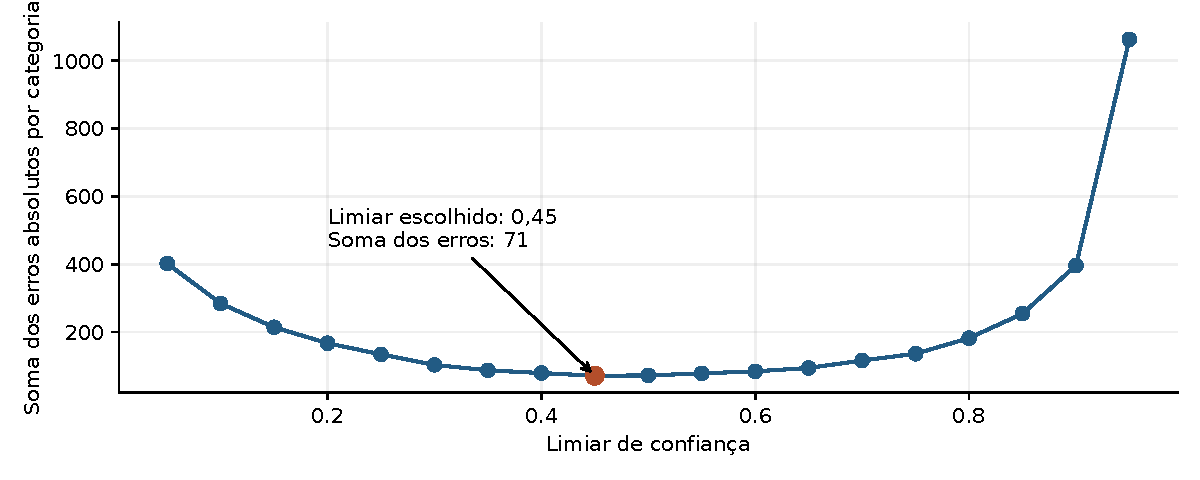
\includegraphics[width=.95\linewidth]{figuras/resultados_calibracao.pdf}
\par\smallskip{\footnotesize Fonte: elaboração própria, com base na calibração no conjunto de validação.\par}
\end{figure}

A escolha anterior ao teste preserva a finalidade desse conjunto: avaliar uma configuração já definida. Ajustar repetidamente o limiar a partir dos erros de teste reduziria a independência dessa avaliação. A revisão visual posterior foi empregada para compreender as falhas, sem modificar o limiar nem recalcular os resultados apresentados neste capítulo.

\vspace{\baselineskip}
\phantomsection
\addcontentsline{toc}{subsection}{4.3 Desempenho na detecção dos instrumentos}
\noindent\textbf{4.3 Desempenho na detecção dos instrumentos}\par
\nobreak\vspace{\baselineskip}\nobreak

Na avaliação padrão de detecção no teste, o modelo alcançou mAP@0,50 de 98,06\% e mAP@0,50:\allowbreak{}0,95 de 86,73\%. O resultado mais alto no primeiro critério mostra que a identificação com sobreposição mínima de 50\% foi mais favorável do que a avaliação que também exige delimitações mais próximas da referência. Assim, o modelo pode localizar a região do instrumento e ainda apresentar diferenças no tamanho ou na posição da caixa.

Para examinar o funcionamento da contagem, a Tabela~\ref{tab:res-deteccao} apresenta a precisão e a revocação calculadas com confiança de 0,45 e sobreposição mínima de 50\%. A precisão informa a proporção de detecções aceitas que corresponderam a objetos da categoria correta. A revocação informa a proporção dos objetos de referência que foi recuperada pelo modelo. Esses valores em um limiar fixo não devem ser confundidos com a precisão média, que considera a ordenação das previsões por confiança.

\begin{table}[htbp]
\centering
\caption{Detecção por categoria no ponto de operação adotado para a contagem}
\label{tab:res-deteccao}
\begin{minipage}{\linewidth}\small\singlespacing
\centering
\begin{tabular}{p{4.1cm}rrrr}
\hline
Categoria & Objetos & Acertos & Precisão (\%) & Revocação (\%) \\
\hline
Pinças & 509 & 497 & 97,26 & 97,64 \\
Tesouras & 451 & 442 & 99,33 & 98,00 \\
Afastadores & 81 & 78 & 91,76 & 96,30 \\
Porta-agulhas & 76 & 71 & 98,61 & 93,42 \\
Cabos de bisturi & 209 & 188 & 92,61 & 89,95 \\
Bicos de aspiração & 21 & 20 & 100,00 & 95,24 \\
Cúpulas & 30 & 30 & 96,77 & 100,00 \\
\hline
\end{tabular}
\par\smallskip\raggedright\footnotesize Fonte: elaboração própria.

Nota: objetos correspondem às anotações de referência utilizadas na avaliação; acertos representam detecções associadas à categoria correta com IoU $\geq 0{,}50$ e confiança $\geq 0{,}45$. Duas classificações incorretas da categoria porta-agulhas são examinadas na Seção~4.6.

\end{minipage}
\end{table}

Os cabos de bisturi apresentaram a menor revocação: 188 dos 209 objetos foram recuperados segundo o critério de correspondência. Também ocorreram 15 detecções incorretas nessa categoria. Nos afastadores, a precisão foi de 91,76\%, com sete detecções incorretas, enquanto três objetos não foram recuperados. Esses resultados indicam dificuldades diferentes: além de deixar de detectar objetos, o modelo pode gerar mais de uma previsão ou atribuir a categoria a uma região que não corresponde a um instrumento desejado.

As tesouras apresentaram precisão de 99,33\% e revocação de 98,00\%, com maior quantidade de objetos de referência do que os bicos de aspiração e as cúpulas. Para estas duas últimas categorias, os resultados favoráveis precisam ser interpretados à luz dos 21 e 30 objetos disponíveis no teste. A precisão de 100\% dos bicos de aspiração significa que não houve detecção incorreta dessa categoria neste conjunto; não significa ausência de falhas em novas situações. Da mesma forma, todas as cúpulas de referência foram recuperadas, mas houve uma detecção adicional incorreta.

\vspace{\baselineskip}
\phantomsection
\addcontentsline{toc}{subsection}{4.4 Contagem total e contagem por categoria}
\noindent\textbf{4.4 Contagem total e contagem por categoria}\par
\nobreak\vspace{\baselineskip}\nobreak

A contagem total coincidiu com a referência em 972 das 1.008 imagens, correspondendo a 96,43\%. Nas demais, houve subcontagem em 21 imagens e sobrecontagem em 15. O erro absoluto médio foi de 0,0536 objeto por imagem, calculado a partir da soma de 54 diferenças absolutas dividida pelas 1.008 imagens. Esse valor é uma média: não representa uma fração física de instrumento em cada fotografia e pode reunir muitos acertos com alguns erros maiores.

Ao exigir simultaneamente a quantidade correta em todas as sete categorias, o número de imagens com acerto diminuiu para 964, ou 95,63\%. Essa exigência corresponde à coincidência do vetor de contagens: além do total, cada posição da lista de quantidades por categoria deve estar correta. A diferença de oito imagens em relação ao acerto total mostra por que contar corretamente o conjunto não garante reconhecer corretamente sua composição. Um objeto atribuído à categoria errada pode preservar o total, mas altera duas posições dessa lista.

A soma dos erros absolutos por categoria foi de 76, equivalente à média de 0,0754 por imagem. Essa medida foi maior do que o erro da contagem total porque não permite compensações entre categorias. Considerando todas as imagens em conjunto, foram previstos 1.367 objetos, dez a menos do que os 1.377 da referência. Contudo, a diferença de dez no total agregado ocultaria erros locais de sentidos opostos. Para a conferência de uma fotografia, a comparação por imagem é mais informativa do que apenas somar todas as previsões do conjunto.



\begin{table}[htbp]
\centering
\caption{Erro absoluto médio da contagem por categoria no conjunto de teste}
\label{tab:res-mae-categorias}

\begin{minipage}{0.98\linewidth}
\singlespacing
\small
\centering

\begin{tabular}{lrrrr}
\hline
Categoria & Imagens positivas & Objetos & MAE geral & MAE positivo \\
\hline
Pinças             & 491 & 509 & 0,0218 & 0,0305 \\
Tesouras           & 340 & 451 & 0,0119 & 0,0294 \\
Afastadores        & 25  & 81  & 0,0079 & 0,3200 \\
Porta-agulhas      & 75  & 76  & 0,0060 & 0,0800 \\
Cabos de bisturi   & 191 & 209 & 0,0258 & 0,1309 \\
Bicos de aspiração & 20  & 21  & 0,0010 & 0,0500 \\
Cúpulas            & 30  & 30  & 0,0010 & 0,0000 \\
\hline
\end{tabular}

\par
\vspace{0.35em}
\raggedright
\footnotesize

Fonte: elaboração própria, a partir dos registros de avaliação do modelo (2026).

\par\vspace{0.25em}

\textit{Nota:} imagens positivas representam fotografias com pelo menos um objeto de referência da categoria. O MAE geral foi calculado sobre as 1.008 imagens de teste, incluindo aquelas sem objetos da categoria. O MAE positivo considera somente as imagens positivas da respectiva categoria. Ambos estão expressos em objetos por imagem.

\end{minipage}
\end{table}



Os cabos de bisturi apresentaram o maior MAE geral (0,0258), seguidos pelas pinças (0,0218). Entretanto, quando o cálculo considera somente as imagens positivas de cada categoria, destacam-se os afastadores, com MAE de 0,3200 em 25 imagens, e os cabos de bisturi, com 0,1309 em 191 imagens. Essa diferença evidencia como a baixa frequência de uma categoria pode reduzir seu erro médio quando todas as imagens do teste são consideradas. No caso das cúpulas, o MAE positivo foi nulo, enquanto o MAE geral foi de 0,0010, pois ocorreu uma previsão indevida em uma imagem sem objetos dessa categoria. Portanto, os dois indicadores são complementares: o MAE positivo caracteriza os erros de contagem nas imagens que contêm a categoria, enquanto o MAE geral também considera previsões indevidas em imagens nas quais ela está ausente. A quantidade desigual de imagens positivas deve ser considerada na comparação entre as categorias.


Além disso, a contagem correta não assegura uma delimitação correta. Uma previsão pode produzir o número esperado de objetos, mas apresentar uma caixa com sobreposição insuficiente em relação à referência. A avaliação conjunta das contagens e das detecções evita tratar esses casos como equivalentes a uma identificação inteiramente correta.

\vspace{\baselineskip}
\phantomsection
\addcontentsline{toc}{subsection}{4.5 Origem das imagens e quantidade de objetos na cena}
\noindent\textbf{4.5 Origem das imagens e quantidade de objetos na cena}\par
\nobreak\vspace{\baselineskip}\nobreak

A Tabela~\ref{tab:res-origem} separa os resultados pela origem das imagens. O acerto da contagem total foi de 98,39\% nas fotografias do HU-UEL e de 93,99\% nas imagens da internet. A coincidência das quantidades em todas as categorias também foi maior no subconjunto hospitalar.

\begin{table}[htbp]
\centering
\caption{Resultados de contagem por origem das imagens de teste}
\label{tab:res-origem}
\begin{minipage}{\linewidth}\small\singlespacing\centering
\begin{tabular}{p{2.3cm}rrrrr}
\hline
Origem & Imagens & Objetos & Total correto & Vetor correto & MAE total \\
\hline
HU-UEL & 559 & 647 & 98,39\% & 98,21\% & 0,0197 \\
Internet & 449 & 730 & 93,99\% & 92,43\% & 0,0958 \\
Conjunto & 1.008 & 1.377 & 96,43\% & 95,63\% & 0,0536 \\
\hline
\end{tabular}
\par\smallskip\raggedright\footnotesize Fonte: elaboração própria. Total correto e vetor correto representam proporções de imagens. MAE total: erro absoluto médio da quantidade total por imagem.
\end{minipage}
\end{table}

Essa diferença não demonstra que a origem hospitalar, isoladamente, tenha causado o melhor desempenho. Os subconjuntos diferem na composição de categorias, no número de objetos, no enquadramento e nas condições de captura. As fotografias hospitalares também podem compartilhar características visuais das sessões de aquisição presentes na base. Portanto, o resultado descreve o conjunto reservado para teste, sem equivaler a uma avaliação prospectiva em novos dias, ambientes ou rotinas de trabalho.

Há ainda uma restrição de cobertura: o subconjunto de teste do HU-UEL não contém cabos de bisturi anotados. Consequentemente, os resultados dessa categoria são provenientes das imagens da internet e não demonstram seu desempenho em fotografias hospitalares. Para porta-agulhas, bicos de aspiração e cúpulas do HU-UEL, foram avaliados, respectivamente, 18, 15 e 28 objetos, todos recuperados sem previsões adicionais dessas categorias nesse subconjunto. Embora favoráveis, essas observações abrangem amostras pequenas e condições limitadas de aquisição.

A quantidade de objetos na cena revela outra diferença importante. Das 1.008 imagens de teste, 845, ou 83,83\%, contêm apenas um objeto. Nesse grupo, a contagem total foi correta em 839 imagens, correspondendo a 99,29\%. Nas cenas com dois ou três objetos, o acerto foi de 84,31\%; nas cenas com quatro ou mais, foi de 78,43\%, como mostra a Figura~\ref{fig:res-cenas}.

\begin{figure}[htbp]
\centering
\caption{Acerto da contagem total conforme a quantidade de objetos de referência na cena}
\label{fig:res-cenas}
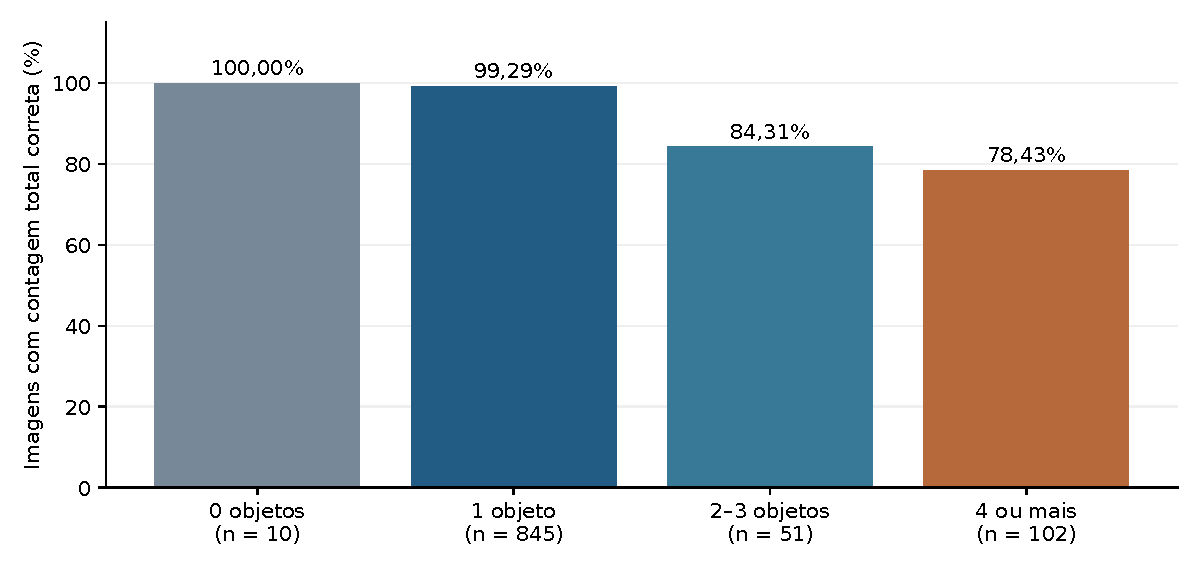
\includegraphics[width=.96\linewidth]{figuras/resultados_contagem_cenas.pdf}
\par\smallskip{\footnotesize Fonte: elaboração própria. O valor de $n$ indica a quantidade de imagens em cada grupo.\par}
\end{figure}

O erro absoluto médio também aumentou entre esses grupos: foi de 0,0107 nas imagens com um objeto, 0,1765 nas imagens com dois ou três e 0,3529 nas imagens com quatro ou mais. Esses números mostram uma associação entre cenas com mais objetos e maior dificuldade no conjunto avaliado. Como a composição das categorias e as condições das fotografias também variam, não é possível atribuir toda a diferença apenas ao número de instrumentos.

O grupo com quatro ou mais objetos reúne 102 imagens, das quais 100 possuem quatro objetos, uma possui cinco e uma possui dez. Assim, ele representa principalmente cenas com quatro instrumentos, e não bandejas completas com grande concentração de itens. As dez imagens sem objetos apresentaram contagem zero corretamente. Esse resultado é útil para verificar bandejas vazias, mas não demonstra que o modelo rejeitaria qualquer objeto estranho ou instrumento fora das categorias de interesse.

\vspace{\baselineskip}
\phantomsection
\addcontentsline{toc}{subsection}{4.6 Análise visual dos acertos e das falhas}
\noindent\textbf{4.6 Análise visual dos acertos e das falhas}\par
\nobreak\vspace{\baselineskip}\nobreak

Para compreender os resultados numéricos, foram examinadas visualmente 62 imagens: 30 selecionadas entre os maiores erros de contagem por categoria, duas com contagem correta e falha de correspondência espacial, 20 casos de acerto sorteados e dez imagens sem objetos. Essa seleção reúne situações úteis para análise, mas não constitui uma amostra aleatória de todo o teste. Portanto, a frequência de uma dificuldade nessa revisão não pode ser generalizada para todas as imagens.

Nos exemplos de acerto, as caixas delimitaram os instrumentos e receberam as categorias esperadas, inclusive em fotografias do HU-UEL. Nas falhas, foram observadas situações com instrumentos próximos ou sobrepostos, objetos visualmente semelhantes e regiões de baixo contraste. Essas observações ajudam a formular explicações para os erros, mas não isolam experimentalmente a contribuição de cada fator.

A Figura~\ref{fig:res-exemplos} apresenta dois casos. Na imagem dos afastadores Farabeuf, quatro objetos de referência resultaram em sete previsões. A proximidade e a sobreposição dos instrumentos dificultam distinguir suas partes e associá-las a um único objeto. No segundo exemplo, havia um cabo de bisturi de interesse e cinco lâminas; o modelo contou cinco objetos como cabos, incluindo quatro lâminas indevidamente. Esse caso mostra que uma categoria pode receber previsões de objetos com partes visualmente semelhantes, ainda que esses objetos não devam participar da contagem.

\begin{figure}[H]
\centering
\caption{Exemplos de sobrecontagem em afastadores e de confusão entre cabo de bisturi e lâminas}
\label{fig:res-exemplos}

\begin{minipage}[t]{0.49\linewidth}
\centering
{\small (a) Farabeuf: referência\par}
\vspace{0.2em}
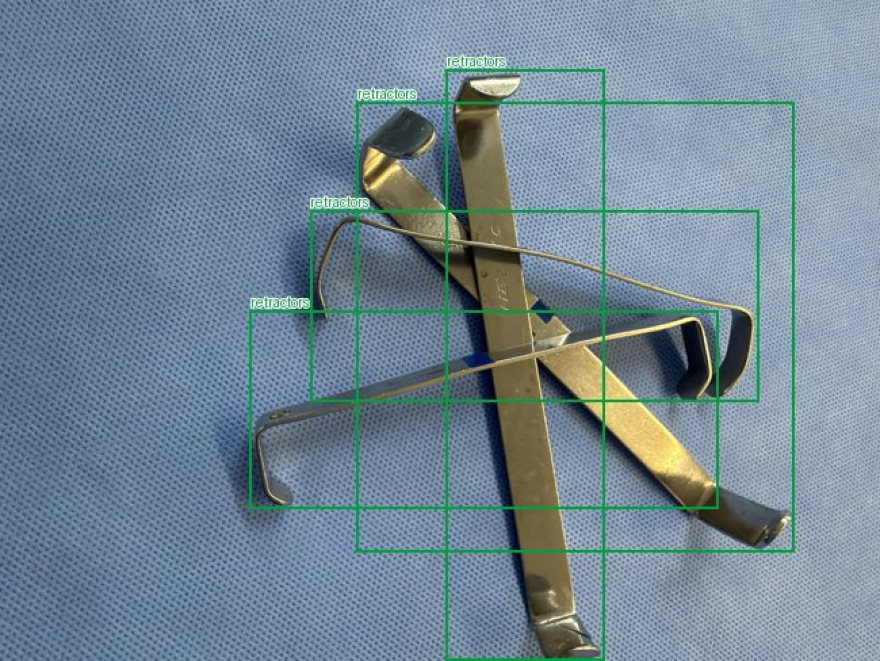
\includegraphics[width=\linewidth]{figuras/fig10_a_farabeuf_referencia.png}
\end{minipage}\hfill
\begin{minipage}[t]{0.49\linewidth}
\centering
{\small (b) Farabeuf: predição\par}
\vspace{0.2em}
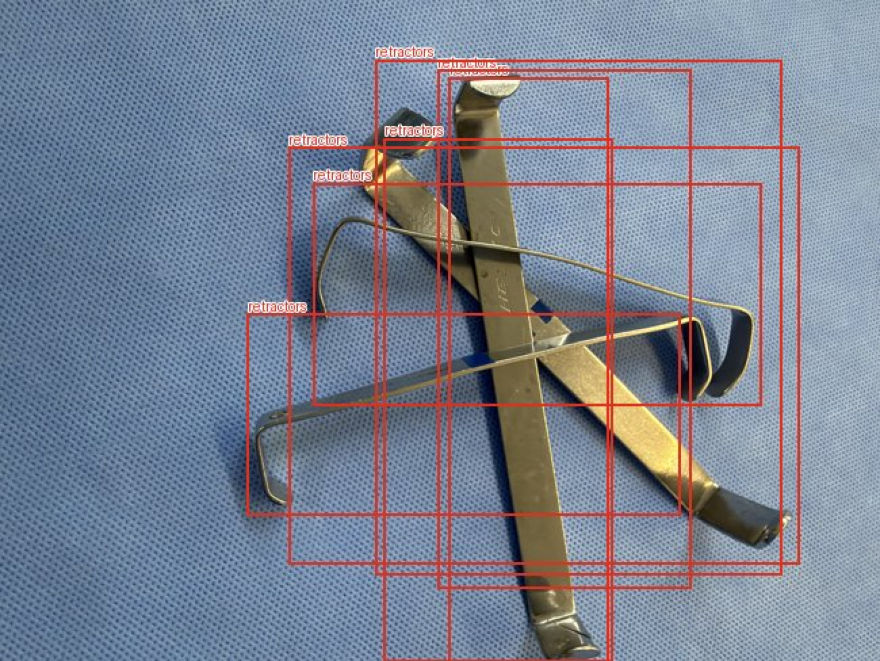
\includegraphics[width=\linewidth]{figuras/fig10_b_farabeuf_predicao.png}
\end{minipage}

\vspace{0.35cm}

\begin{minipage}[t]{0.49\linewidth}
\centering
{\small (c) Cabo e lâminas: referência\par}
\vspace{0.2em}
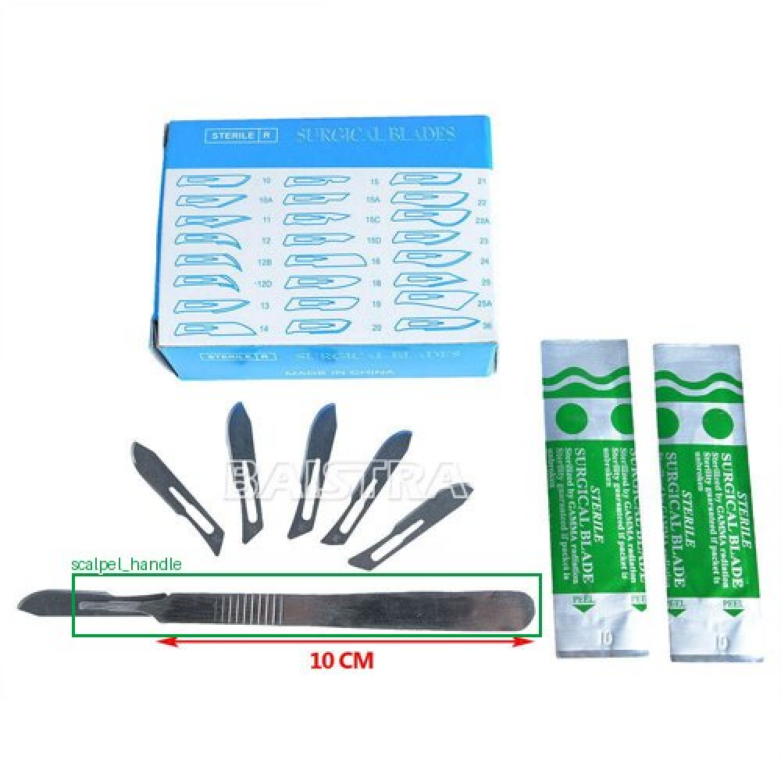
\includegraphics[width=\linewidth]{figuras/fig10_c_cabo_referencia.png}
\end{minipage}\hfill
\begin{minipage}[t]{0.49\linewidth}
\centering
{\small (d) Cabo e lâminas: predição\par}
\vspace{0.2em}
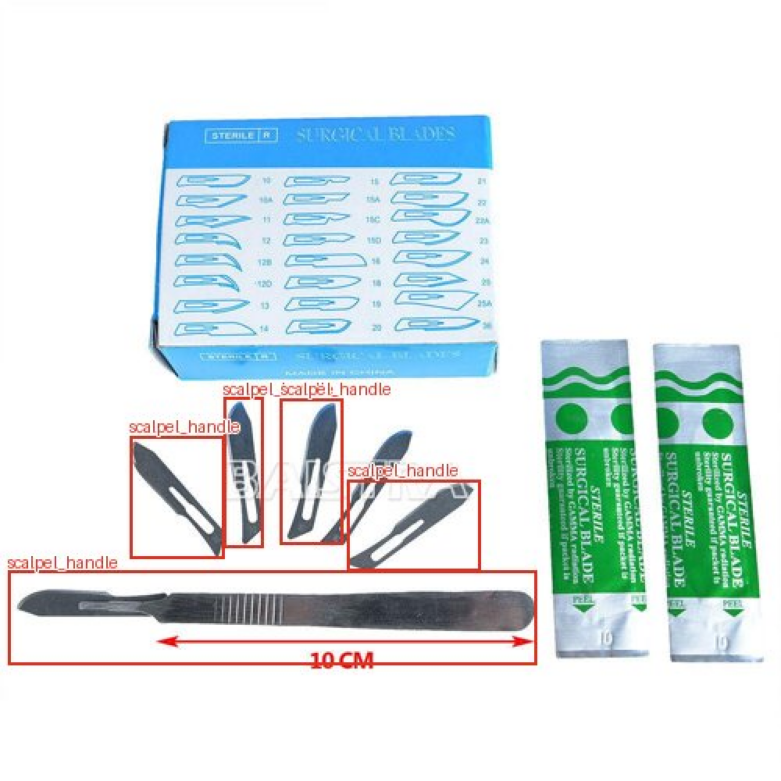
\includegraphics[width=\linewidth]{figuras/fig10_d_cabo_predicao.png}
\end{minipage}

\par\smallskip
{\footnotesize\raggedright
Fonte: elaboração própria, a partir das imagens do conjunto de teste e das saídas do modelo. Em (a) e (c), as caixas de referência aparecem em verde; em (b) e (d), as previsões aparecem em vermelho. Os identificadores em inglês correspondem às categorias utilizadas no processamento.\par}
\end{figure}

Também ocorreram omissões em fotografias com vários cabos de bisturi. Em um caso com cinco cabos lado a lado, foram detectados somente os dois externos. Em outro, com dez objetos de referência, foram previstos três. Esses exemplos ajudam a explicar por que a diferença entre o total previsto e o total de referência pode ser elevada em algumas imagens, apesar do erro médio reduzido no conjunto completo.


A revisão visual identificou ainda duas classificações incorretas nas anotações de referência: duas imagens de pinça Kelly reta haviam sido classificadas como porta-agulhas. Em ambos os casos, o modelo produziu uma previsão da categoria pinças, compatível com a identificação visual confirmada pela enfermeira colaboradora. Os resultados apresentados foram preservados conforme as anotações utilizadas na avaliação. Como análise de sensibilidade, considerando a correção dessas duas referências e mantendo as detecções e os 71 acertos originais da categoria porta-agulhas, sua revocação passaria de 93,42\% (71/76) para aproximadamente 95,95\% (71/74). Esse cálculo não constitui uma reavaliação completa das métricas, mas demonstra que parte do erro registrado decorre da referência utilizada, e não necessariamente de uma falha de identificação do modelo.

\vspace{\baselineskip}
\phantomsection
\addcontentsline{toc}{subsection}{4.7 Tempo de processamento e alcance dos resultados}
\noindent\textbf{4.7 Tempo de processamento e alcance dos resultados}\par
\nobreak\vspace{\baselineskip}\nobreak

O tempo de processamento foi medido em 50 imagens de teste, após três chamadas de aquecimento, com uma imagem por chamada e sincronização do processamento no dispositivo. A medição da chamada completa incluiu a leitura da imagem, o pré-processamento, a inferência e o pós-processamento. A média foi de 29,24 ms por imagem e a mediana de 24,22 ms. O percentil 95 foi de 48,81 ms, indicando que aproximadamente 95\% dos tempos medidos ficaram abaixo desse valor. O maior tempo observado foi de 281,13 ms, evidenciando que a duração não foi constante.

Esses valores sugerem rapidez para processar fotografias nas condições avaliadas. Entretanto, não incluem o tempo necessário para organizar os instrumentos, capturar a fotografia, transferi-la e conferir o resultado em uma aplicação completa. Também não equivalem a uma taxa de quadros validada em vídeo contínuo. O ganho de tempo na rotina hospitalar dependeria dessas etapas e exigiria uma avaliação própria do fluxo de trabalho.

A literatura oferece exemplos de detecção de instrumentos em condições distintas. \textcite{deol2024} avaliaram uma abordagem baseada em YOLOv9 com imagens contendo combinações de instrumentos, inclusive sobreposição e cenas com até 34 objetos. Esse tipo de cenário evidencia a importância de avaliar conjuntos mais densos. Contudo, diferenças no número de categorias, nas imagens, nas divisões dos dados e no protocolo impedem interpretar os valores de desempenho dos dois estudos como uma comparação direta de superioridade entre modelos.

A separação de imagens relacionadas entre treino, validação e teste também interfere na confiabilidade da avaliação. \textcite{kapoor2023} discutem como o vazamento de informação pode produzir estimativas excessivamente favoráveis em pesquisas com aprendizado de máquina. Nesta pesquisa, foram empregados agrupamentos e verificações de similaridade para reduzir esse risco. Esses procedimentos, porém, não demonstram independência completa entre todas as sessões de aquisição nem eliminam semelhanças que possam ter permanecido entre fotografias. Uma avaliação posterior com novas sessões de captura constitui uma forma importante de examinar essa limitação.

O experimento avaliou uma única configuração do YOLO26n, de modo que seus resultados não estabelecem superioridade em relação a outras variantes ou modelos. Além disso, uma operação do dispositivo MPS não dispunha de implementação determinística, o que limita a reprodução numérica exata mesmo com a semente fixada.

Os resultados sustentam uma viabilidade técnica inicial da detecção e da contagem por categorias gerais nas condições examinadas, especialmente em imagens com um instrumento e nas fotografias hospitalares representadas no teste. Essa conclusão é mais restrita do que afirmar que o sistema está pronto para conferir uma caixa cirúrgica completa. A redução do acerto nas cenas com vários objetos, a cobertura desigual das categorias e as falhas observadas em instrumentos próximos mostram a necessidade de ampliar a avaliação antes de propor seu uso como apoio à rotina. Assim, a principal contribuição desta etapa é demonstrar o potencial da abordagem e identificar, com dados de detecção e contagem, as condições que ainda exigem melhoria.

\endgroup
